In this section, we will analyse the behavior of the system with the variety of all read requests and expose the system to the factors listed in the Section \ref{tab:request_factors}, i.e., waiting between requests, load distribution, and connection pool.
  
  
  \subsection{With variety}
  
  After in the previous section we understood how the system reacts if there is only one type of request being executed, in this section we will analyse its behavior if there are several types of requests being executed, more specifically, all the reading requests listed in Table \ref{tab:type_requests}. Furthermore, we will not consider any restrictions on the way requests are made, nor any changes in the way the system handles them, since the results of the tests in this section will be used as a comparison to the remaining ones in this performance evaluation.
  
  
  \subsubsection{Throughput}
  
  It is to be expected that the evaluation of this metric will only corroborate the conclusions drawn in individual testing, since the only change from that testing is the request variety.
  
    \begin{figure}[H]
    \centering
    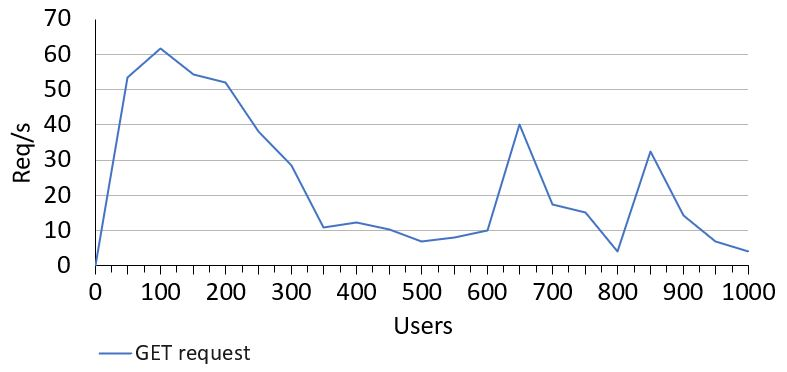
\includegraphics[width=.8\textwidth]{img/performance_evaluation/normal.JPG}
    \caption{\label{tab:throughput_normal}Throughput}
  \end{figure}
  
  We can then prove what we expected from the graph in Figure \ref{tab:throughput_normal}, that is, that the 200 users remains the point at which a significant drop in the number of requests executed per second begins to appear. Moreover, the large amplitude between requests exists from the 200 concurrent user mark onwards, with the same irregular peaks present in the individual case.
  
  Next, we present the table \ref{tab:geral_norma} with general information regarding the number of requests executed per second, as well as other information that may be useful for making comparisons with other tests.
  
  \newpage
  
  \begin{table}[h]
    \centering
    \begin{tabular}{|>{\centering\arraybackslash}p{2.5cm}|>{\centering\arraybackslash}p{2cm}|>{\centering\arraybackslash}p{4cm}|>{\centering\arraybackslash}p{1.5cm}|} 
      \hline
      \textbf{\# Requests} & \textbf{\# Fails} & \textbf{Average size (bytes)} & \textbf{RPS} \\ 
      \hline
      8096 & 355 & 50200 & 28.8  \\ 
      \hline
    \end{tabular}
    \caption{\label{tab:geral_norma}Request statistics}
  \end{table}
  
  Of the 8096 requests made to the system, 335 fail (note that this failure is not harmful to the system), that is, 335 exceed the timeout in terms of time for the server to respond to something, which is due to the higher traffic of requests, but we will address more clearly the occasions when this happens afterwards.
  
  \subsubsection{Response Time}
  
  For this metric, we will look at the median response time, i.e., the time value that separates the highest and lowest half of our sample of server response times to requests made to it, and the 95\% percentile, i.e., how long it takes the server to respond to requests 95 percent of the time. It is to be expected that from 200 users onwards, these values will start to increase with some significance, and that, as with throughput, there will also be a certain range between users and irregular peaks.
  
  \begin{figure}[H]
    \centering
    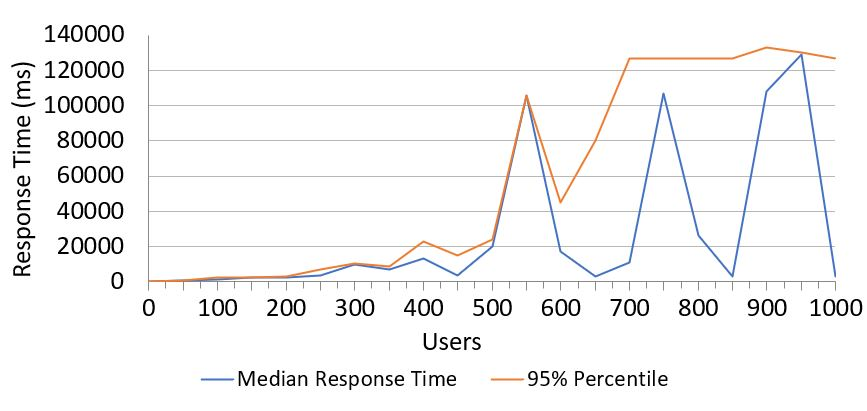
\includegraphics[width=1\textwidth]{img/performance_evaluation/normal_time.JPG}
    \caption{\label{tab:time_normal}Response Time}
  \end{figure}
  
  \newpage
  
  Looking at the graph in figure \ref{tab:time_normal}, we can then confirm the expected: 
  
  \begin{itemize}
      \item Until the 200 users mark the system responds in an acceptable way, more specifically, the server has a median of 2430 ms and 95\% of the time it can respond in a maximum of 3170 ms to the requests that are made to it. However, although we take into account that most of the requests are somewhat heavy, 3s is something that we believe we can improve;
      \item After 200 concurrent users, the system begins to behave somewhat unpredictably, however, always in an unbearable way. It is worth mentioning the 500 users mark, since from that point on, the system starts to suffer more aggressively, since it goes from being able to respond 95\% of the time in a maximum of 24000 ms to values higher than 100000s, that is, an increase of more than 400\%, which results in the growth of faults in the system, since the timeout used for read requests is 5s.
  \end{itemize}
  
 To add an interesting statistic to compare later, the average response time was 9156 ms.
  
  \subsubsection{CPU and Disk Utilisation}
  
  For this evaluation, with the help of the Linux iostat command, we will make an analysis of the percentage of CPU usage that occurred during the execution at the user level (i.e. application) and, when it comes to disk usage, we chose to compile the information (tps - number of transfers per second to the device,  kb\_read/s - amount of data read from the device, kb\_wrtn/s - amount of data written to the from the device) of the devices into one, these being sda, sdb and sdd, which were the ones that showed changes during the execution of the test. As far as the CPU is concerned, since we have 80 CPUs, the result is an average of the usage of each one.
  
  We provide the above information for 100, 500 and 1000 users in the Table \ref{tab:cpu_normal}, i.e. the CPU and disk utilisation from the initial moment up to 100 users, then the utilisation between 100 and 500 users, and finally between 500 and 1000.
 
  \newpage

\begin{table}[h!]
\centering
\begin{tabular}{|c|c|c|c|c|} 
\hline
\multirow{2}{*}{\textbf{Users }} & \multirow{2}{*}{\textbf{~\%CPU}} & \multicolumn{3}{c|}{\textbf{Devices}}                     \\ 
\cline{3-5}
                                 &                                  & \textbf{tps} & \textbf{kB\_read/s} & \textbf{kB\_wrtn/s}  \\ 
\hline
100  & 1,5 & 2,1  & 0  &  36,2                  \\ 
\hline
500  & 0,8 & 2,2 & 0 & 35,5                   \\ 
\hline
1000 & 0,6 & 2,3 & 0 & 27,8                 \\ 
\hline
\end{tabular}\caption{\label{tab:cpu_normal}CPU and Disk utilisation}
\end{table}


This way we realize that the fact that \textit{Locust} uses only one process results in almost zero CPU usage and, in turn, Disk usage is also residual. Note that both metrics are influenced, in a minimal way, by other processes than those used by the tests or the server. Furthermore, no information is read from the devices, since it is already in the CPU cache, loaded at the beginning of the test.
  
  
  \subsection{With variety and waiting between requests}
  
  At this point, let's evaluate the system taking into account that there are waits between requests. To do this, we changed our script by adding an attribute that \textit{Locust} provides for the User class, more specifically, wait\_time, which introduces a delay after the execution of each task.
    
  \begin{verbatim}
   wait_time = constant_throughput(0.25)
  \end{verbatim}
  
  The above assignment guarantees that each User runs a task 0.25 times per second, i.e., 1 task every 4 seconds, which seems to us a realistic estimate of system usage by a client on average.

  \subsubsection{Throughput}
  
  Something we can expect before testing this metric is that the initial growth of requests may not be as steep as for a no-wait test. As such, it should also have an influence on the speed with which the system will reach the optimal concurrency situation, more specifically, it should take longer to reach that state.

  \begin{figure}[H]
    \centering
    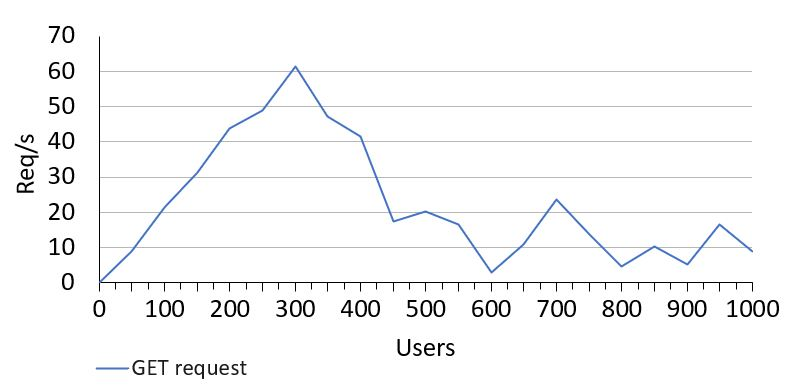
\includegraphics[width=.8\textwidth]{img/performance_evaluation/wait.JPG}
    \caption{\label{tab:thorughput_wait}Throughput with waiting between requests}
  \end{figure}
  
  From the Figure \ref{tab:thorughput_wait} we can conclude the following:
  
  \begin{itemize}
      \item The wait between requests causes what would be expected, that is, a less gradual growth until diminishing returns are reached, which in this case we can point to end up at 400 users. This is good news, since by considering a case closer to reality, we managed to double the ideal competition limit;
      \item Passing the mark of the ideal number of concurrent users, in contrast to the large range between requests when there is no wait, here the range, while still existing, exists to a lesser extent.
  \end{itemize}
  
  From the same test performed for the elaboration of the graph of the Figure \ref{tab:thorughput_wait}, we were able to extract information regarding the total values of the requests made, among other values. We present this information available in the following Table \ref{tab:geral_wait}.
  
  \begin{table}[h]
    \centering
    \begin{tabular}{|>{\centering\arraybackslash}p{2.5cm}|>{\centering\arraybackslash}p{2cm}|>{\centering\arraybackslash}p{4cm}|>{\centering\arraybackslash}p{1.5cm}|} 
      \hline
      \textbf{\# Requests} & \textbf{\# Fails} & \textbf{Average size (bytes)} & \textbf{RPS} \\ 
      \hline
      5967 & 237 & 51139 & 21.6  \\ 
      \hline
    \end{tabular}
    \caption{\label{tab:geral_wait}Request statistics with waiting between requests}
  \end{table}
  
   We then see that fewer requests are made in total relative to a system without waits, which makes perfect sense. Without wanting to fall into redundancy, more waiting, fewer requests, however, this is not something negative, just a consequence of the reality of a system in which all users are not constantly making requests.
  
  \subsubsection{Response Time}
  
  Now, we try to understand how the system performs in terms of time to process and respond to a request. We again expect that, just as happened with the throughput, the response times should start to increase later, less gradually.
  
  \begin{figure}[H]
    \centering
    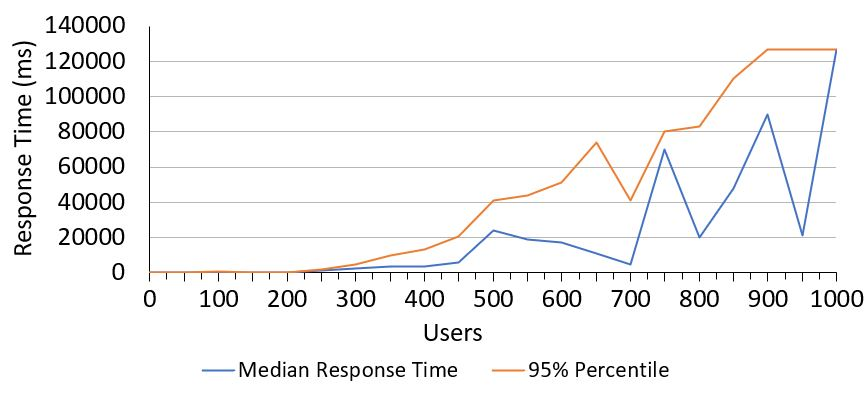
\includegraphics[width=1\textwidth]{img/performance_evaluation/wait_time.JPG}
    \caption{\label{tab:time_wait}Response time with waiting between requests}
  \end{figure}
  
  Thus, with the help of Figure \ref{tab:time_wait} we can confirm what we theorize. On the one hand, the 95\% percentile and the median start showing signs of increase even before 200 users in a system without waits between requests, and the 95\% percentile reaches the maximum value of 127000 ms at the 700 users mark. On the other hand, for the system we are considering in this subsection the median starts to increase considerably after 450 users, and the 95\% percentile start increasing after 300 users and reaches the maximum value at the 900 users mark. 
  From the same test, we also took the average response time, this was 10190 ms.
  
  \subsubsection{CPU and Disk Utilisation}
  
  We expect that, unlike the first scenario, there will be a greater CPU usage after 100 users, since until this mark the ideal number of concurrent users in the system has not yet been reached. Regarding the use of the Disk, we believe that it will again be residual.

\newpage

\begin{table}[h!]
\centering
\begin{tabular}{|c|c|c|c|c|} 
\hline
\multirow{2}{*}{\textbf{Users }} & \multirow{2}{*}{\textbf{~\%CPU}} & \multicolumn{3}{c|}{\textbf{Devices}}                     \\ 
\cline{3-5}
                                 &                                  & \textbf{tps} & \textbf{kB\_read/s} & \textbf{kB\_wrtn/s}  \\ 
\hline
100  & 0,5 & 3,2  & 0  &  34,4                   \\ 
\hline
500  & 1,1 & 2,5 & 0 & 33,5                    \\ 
\hline
1000 & 0,4 & 2,1 & 0 & 23,9                 \\ 
\hline
\end{tabular}\caption{\label{tab:cpu_waiting}CPU and Disk utilisation}
\end{table}

  We confirm the expected through Table \ref{tab:cpu_waiting}.
 

  \subsection{With variety, waiting between requests and distributed load}

  We now consider two factors, namely, the wait between requests, since it showed to be a factor to consider in a realistic case, and, additionally, the load distribution that \textit{Locust} allows.
  
  While a single process running Locust can simulate a significant number when it comes to throughput, for more complex or higher load tests, scaling to multiple processes, and even multiple machines, is something to strongly consider. In our case, since we have hardware with higher capacity than usual, we will explore this feature. To do so, we use the same script as in the previous section, we just modify the way we run it, as well as the number of instances created, that is, we run one instance of Locust in one terminal using the master flag and 40 other instances (we use 40 since, typically, the Locust team suggests using one worker instance per processor core) in different terminals using the worker flag. The master instance tells the workers when to stop or start and does not run Users, while the workers run Users and send back statistics to the master.
  
  \subsubsection{Throughput}
  
  For this metric, we think that the distribution load will result in better overall throughput, because the process cores will be less heavy than a single would be, and for that very reason, probably the moment of diminishing returns will last longer.
  
    \begin{figure}[H]
    \centering
    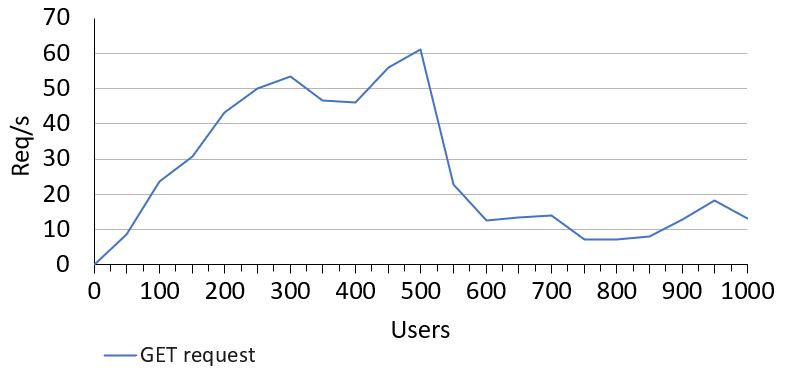
\includegraphics[width=.8\textwidth]{img/performance_evaluation/distributed.JPG}
    \caption{\label{tab:throughput_dist_load}Throughput with waiting between requests and distributed load}
  \end{figure}
  
  Analysing Figure \ref{tab:throughput_dist_load} we conclude that: 
  
  \begin{itemize}
      \item Our predictions were true, that is, the moment of diminishing returns lasts a little longer, from 200 (as in the test of waits between requests) to 500 concurrent users, which is a record number within the tests we ran;
      \item Similar to the test in the previous section, the range is smaller than the initial tests due to the wait, which allows to have fewer peaks.
  \end{itemize}

  More general statistics regarding the response to requests are presented below in Table \ref{tab:geral_dist_load}.
  
  \begin{table}[h]
    \centering
    \begin{tabular}{|>{\centering\arraybackslash}p{2.5cm}|>{\centering\arraybackslash}p{2cm}|>{\centering\arraybackslash}p{4cm}|>{\centering\arraybackslash}p{1.5cm}|} 
      \hline
      \textbf{\# Requests} & \textbf{\# Fails} & \textbf{Average size (bytes)} & \textbf{RPS} \\ 
      \hline
      8342 & 68 & 54369 & 29.4  \\ 
      \hline
    \end{tabular}
    \caption{\label{tab:geral_dist_load}Request statistics with waiting between requests and distributed load}
  \end{table}
  
  So we broke another record, this time for the total number of requests answered, although it is residual. On the contrary, we managed to decrease the number of failures, which is the result of an improved system capacity, and now, in the analysis of response times, we will understand why.
  
  \subsubsection{Response Time}
  
  In the analysis of this metric we expect to see a lower median response time, and consequently fewer peaks relative to the previous tests due to the removal of the overhead from one process, spreading it across multiples. Also, for the 95\% percentile, we expect that it will not reach stabilization, since it would take more users for that moment to happen.
  
  \begin{figure}[H]
    \centering
    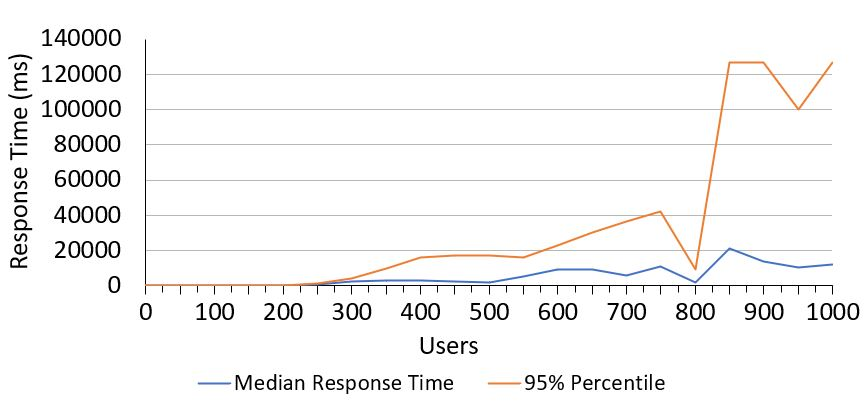
\includegraphics[width=1\textwidth]{img/performance_evaluation/distributed_time.JPG}
    \caption{Response time with waiting between requests and distributed load}
  \end{figure}
  
  Observing the graph in the figure above, we draw the following conclusions:
  
  \begin{itemize}
      \item The median remained until 1000 users without significant variations in its amplitude compared to the other tests, nor did we detect any peak of relevance. In addition, we can observe that the median, as for the previous situations, started to increase with greater intensity from the ideal number of concurrent users (500), this makes sense, since a lower ability to deal with concurrency results in a longer time to respond to requests;
      \item The fact that the median is below 5000s more than half the time explains the low number of failed requests, which is also positive to draw from this metric;
      \item For the 95\% percentile, we can confirm that it effectively does not stabilize at any maximum, and so we can say with certainty that it would take a few more users for this to happen.
  \end{itemize}
  
  We also took the average response time from the same test, this was 5684 ms.
  
  \subsubsection{CPU and Disk Utilisation}
  
  We anticipate that the load distribution will increase CPU usage in percentage, however, we are unable to predict how much the increase will be. Furthermore, we believe that Disk usage will again be residual. We present the relative information in the Table \ref{tab:cpu_dist}.


\begin{table}[h!]
\centering
\begin{tabular}{|c|c|c|c|c|} 
\hline
\multirow{2}{*}{\textbf{Users }} & \multirow{2}{*}{\textbf{~\%CPU}} & \multicolumn{3}{c|}{\textbf{Devices}}                     \\ 
\cline{3-5}
                                 &                                  & \textbf{tps} & \textbf{kB\_read/s} & \textbf{kB\_wrtn/s}  \\ 
\hline
100  & 9,8 & 3,1  & 0  &  32,7                   \\ 
\hline
500  & 10,2 & 2,3 & 0 & 46,2                    \\ 
\hline
1000 & 8,6 & 1,9 & 0 & 35,5                 \\ 
\hline
\end{tabular}\caption{\label{tab:cpu_dist}CPU and Disk utilisation}
\end{table}

  For this scenario, we also ran the Linux top command to get a sense of the CPU utilisation of each processor involved in the testing, and realised that on average each processor was using 20\% of its capacity.

  The CPU utilisation increases about 10 times, which we can explain by the following: each processor uses on average one fifth of its capacity, and since we use 40 processors in the load distribution, which corresponds to half of the possible CPUs, that is, 50\% of the maximum machine capacity, then we conclude that on average the total usage should be:
  
  \begin{verbatim}
      %CPU = (0,2 * 0,5) * 100 % = 10 %
  \end{verbatim}
  
  \subsection{With variety, waiting between requests, distributed load and connection pool}
  
  In addition to the factors considered earlier in this section, we will now add a connection pool, a configuration enabled by \textit{\gls{ckan}}, which uses \textit{SQLAlchemy} (a \textit{Python} \textit{SQL} toolkit and Object Relational Mapper that gives application developers the full power and flexibility of \textit{SQL}) to take advantage of this.
  
  The connection pool technique is used to keep long-running connections in memory for efficient reuse. In addition, it provides management of the total number of connections that the system must use concurrently. To do this we had to add to our \textit{\gls{ckan}} configuration file:
  
  \begin{verbatim}
   sqlalchemy.pool_size = 40
   sqlalchemy.max_overflow = 20
  \end{verbatim}
  
  So we have a pool with size 40, i.e. the number of core processors in our machine, and we allow 20 more connections to be used if necessary, which gives a total of 60 connections, and does not jeopardize the full utilisation of our hardware.
  
  \subsubsection{Throughput}
  
  Regarding this metric, we expect similar behavior to the previous case, but that the better management by the connection pool may be visible at some point in the test.
  
  \begin{figure}[H]
    \centering
    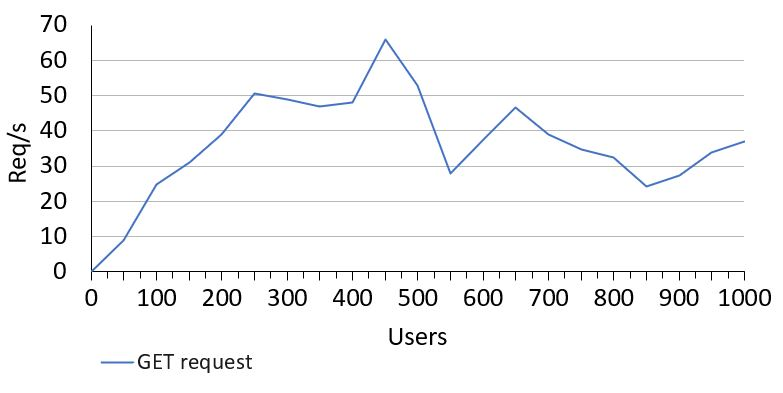
\includegraphics[width=.8\textwidth]{img/performance_evaluation/pool.JPG}
    \caption{Throughput with waiting between requests, distributed load and connection pool}
  \end{figure}
  
  Thus, we confirmed that the system behaves in a similar way, but that after 500 users, which remains as the final moment of diminishing returns, it manages to maintain a throughput between 25 and 45 requests per second until the final moment of the test. This proves the efficiency of the pool management.
  
In order to get a general overview of this test, we can see more information about it in the Table \ref{tab:geral_pool}.

\newpage
  
    \begin{table}[h]
    \centering
    \begin{tabular}{|>{\centering\arraybackslash}p{2.5cm}|>{\centering\arraybackslash}p{2cm}|>{\centering\arraybackslash}p{4cm}|>{\centering\arraybackslash}p{1.5cm}|} 
      \hline
      \textbf{\# Requests} & \textbf{\# Fails} & \textbf{Average size (bytes)} & \textbf{RPS} \\ 
      \hline
      9545 & 71 & 52278 & 35.0  \\ 
      \hline
    \end{tabular}
    \caption{\label{tab:geral_pool}Request statistics with waiting between requests, distributed load and connection pool}
  \end{table}
  
  As we can see, the better management carried out by the connection pool allowed the total number of requests to increase slightly.
  
  \subsubsection{Response Time }
  
  In Figure \ref{tab:pool_time} we will see a graph of the response times for the latter case. At the outset, after improving the throughput, we believe that the response time will also show better results, leveraged by the efficient use of connections.
  
  \begin{figure}[H]
    \centering
    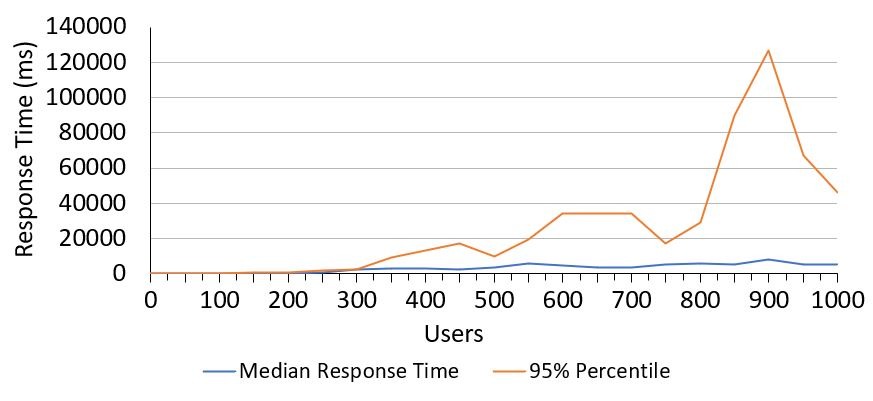
\includegraphics[width=1\textwidth]{img/performance_evaluation/pool_time.JPG}
    \caption{\label{tab:pool_time}Response time with waiting between requests, distributed load and connection pool}
  \end{figure}
  
  Viewing the graph above, we then know that, for the first time, we get a system that can reach 1000 users without ever getting a median greater than 10000ms, demonstrating an almost flat line from start to finish. Certainly, this system can handle an even larger number of users. However, there is no point in exploring further, since it is already unthinkable to even consider requests with a response of about 10s.
  
  As for the average response time, this was 5785 ms.
  
  \subsubsection{CPU and Disk Utilisation}
  
  CPU and Disk usage should be similar to the previous scenario, with a slight difference in CPU usage, which should be more balanced due to the connection pool. The information is presented below in table \ref{tab:cpu_load}.

\begin{table}[h!]
\centering
\begin{tabular}{|c|c|c|c|c|} 
\hline
\multirow{2}{*}{\textbf{Users }} & \multirow{2}{*}{\textbf{~\%CPU}} & \multicolumn{3}{c|}{\textbf{Devices}}                     \\ 
\cline{3-5}
                                 &                                  & \textbf{tps} & \textbf{kB\_read/s} & \textbf{kB\_wrtn/s}  \\ 
\hline
100  & 9,2 & 5,9  & 0  & 65,4                   \\ 
\hline
500  & 10,0 & 2,91 & 0 & 49,3                    \\ 
\hline
1000 & 9,3 & 2,0 & 0 & 38,2                 \\ 
\hline
\end{tabular}\caption{\label{tab:cpu_load}CPU and Disk utilisation}
\end{table}

  We verified what we had predicted, however, the values corresponding to the transfers per second up to 100 users, as well as the number of kB written cause some surprise, and we do not know exactly what caused this increase in relation to the previous scenario.

  \subsection{Summary}
  
  After all the tests of the preliminary case are completed, we compare the former with the latter:
  
  \begin{itemize}
      \item 22 \% gain in the total number of requests executed;
      \item The average response time was almost halved (down about 40\%), which turned out to be the biggest gain;
      \item Decrease of 80\% in the number of failed requests.
  \end{itemize}
  
  We can then state that we have achieved a more efficient system than the one we initially predicted. However, we emphasize that these tests are a pessimistic estimation of how our system will work, mainly due to bandwidth sharing and write requests. We look at this pessimistic estimation as a positive thing, since in a real scenario our system will be able to give an even better answer than the one we presented.
  
  Finally, we conclude that in the realistic scenario that we will present next it will make sense to approach a system like the last one we tested, i.e. with waits between orders, load distribution and connection pool, since they proved to be closer to reality and allowed a better use of the resources we had available.
